%!TEX TS-program = pdflatex
%!TEX root = ../main.tex
%!TEX encoding = UTF-8 Unicode


\section[YOHO model]{YOHO model}

	\begin{frame}{YOHO model}
			
		Presented in 2021\cite{Venkatesh_2022}\dots
		
		\note{
			\dots			
		}		
		
	\end{frame}
	
	\begin{frame}{Output shape}
	
	\begin{figure}
			\centering
			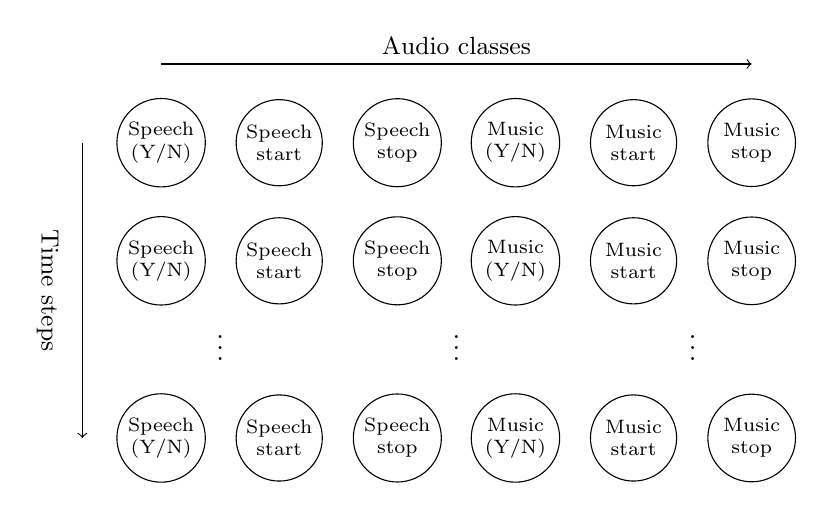
\begin{tikzpicture}
			
				\draw [->,black] (1,6) -- node[midway,above]{\small Audio classes} (8.5,6);
				\draw [->,black] (0,5) -- node[midway,left,below=5pt,sloped]{\small Time steps} (0,1.25);
				
				\node[circle,draw,align=center,inner sep=0pt,text width=1cm,font = {\scriptsize}] at (1,5) {Speech\\(Y/N)};
				\node[circle,draw,align=center,inner sep=0pt,text width=1cm,font = {\scriptsize}] at (2.5,5) {Speech\\start};
				\node[circle,draw,align=center,inner sep=0pt,text width=1cm,font = {\scriptsize}] at (4,5) {Speech\\stop};

				\node[circle,draw,align=center,inner sep=0pt,text width=1cm,font = {\scriptsize}] at (5.5,5) {Music\\(Y/N)};
				\node[circle,draw,align=center,inner sep=0pt,text width=1cm,font = {\scriptsize}] at (7,5) {Music\\start};
				\node[circle,draw,align=center,inner sep=0pt,text width=1cm,font = {\scriptsize}] at (8.5,5) {Music\\stop};


				\node[circle,draw,align=center,inner sep=0pt,text width=1cm,font = {\scriptsize}] at (1,3.5) {Speech\\(Y/N)};
				\node[circle,draw,align=center,inner sep=0pt,text width=1cm,font = {\scriptsize}] at (2.5,3.5) {Speech\\start};
				\node[circle,draw,align=center,inner sep=0pt,text width=1cm,font = {\scriptsize}] at (4,3.5) {Speech\\stop};

				\node[circle,draw,align=center,inner sep=0pt,text width=1cm,font = {\scriptsize}] at (5.5,3.5) {Music\\(Y/N)};
				\node[circle,draw,align=center,inner sep=0pt,text width=1cm,font = {\scriptsize}] at (7,3.5) {Music\\start};
				\node[circle,draw,align=center,inner sep=0pt,text width=1cm,font = {\scriptsize}] at (8.5,3.5) {Music\\stop};

				\node[align=center] at (1.75,2.5) {$\vdots$};
				\node[align=center] at (4.75,2.5) {$\vdots$};
				\node[align=center] at (7.75,2.5) {$\vdots$};

				\node[circle,draw,align=center,inner sep=0pt,text width=1cm,font = {\scriptsize}] at (1,1.25) {Speech\\(Y/N)};
				\node[circle,draw,align=center,inner sep=0pt,text width=1cm,font = {\scriptsize}] at (2.5,1.25) {Speech\\start};
				\node[circle,draw,align=center,inner sep=0pt,text width=1cm,font = {\scriptsize}] at (4,1.25) {Speech\\stop};

				\node[circle,draw,align=center,inner sep=0pt,text width=1cm,font = {\scriptsize}] at (5.5,1.25) {Music\\(Y/N)};
				\node[circle,draw,align=center,inner sep=0pt,text width=1cm,font = {\scriptsize}] at (7,1.25) {Music\\start};
				\node[circle,draw,align=center,inner sep=0pt,text width=1cm,font = {\scriptsize}] at (8.5,1.25) {Music\\stop};

			\end{tikzpicture}
			\caption{The YOHO output shape.}
			\label{fig:YOHOoutput}
		\end{figure}
		
	\end{frame}

	\subsection[Network Architecture]{Network Architecture}
	\begin{frame}{Network Architecture}
		\dots
		
		\note{
			\dots
		}
	\end{frame}

	\subsection[Loss Function]{Loss Function}
	\begin{frame}{Loss Function}
		\begin{equation*}
			\mathcal{L}_{c}(\hat{y},y) = \begin{cases}
			(\hat{y}_1-y_1)^2+\\(\hat{y}_2-y_2)^2+(\hat{y}_3-y_3)^2 &\text{if $y_{1} = 1$}\\
			(\hat{y}_1-y_1)^2, &\text{if $y_1 = 0$}
			\end{cases}
		\end{equation*}
		
		where $y$ and $\hat{y}$ are the ground-truth and predictions respectively. $y_1 = 1$ if the acoustic class is present and $y_1 = 0$ if the class is absent. $y_2$ and $y_3$, which are the start and endpoints for each acoustic class are considered only if $y = 1$.
		In other words, $(\hat{y}_1-y_1)^2$ corresponds to \textbf{the classification loss} and $(\hat{y}_2-y_2)^2+(\hat{y}_3-y_3)^2$ corresponds to \textbf{the regression loss}.
		\note{
			\dots
		}
	\end{frame}
	
	\subsection[Other Details]{Other Details}
	\begin{frame}{Other Details}
		\dots
		
		\note{
			\dots
		}
	\end{frame}


\section[Proposed improvements]{Proposed improvements}

	\begin{frame}{Proposed improvements}
		\dots
		
		\note{
			\dots			
		}		
		
	\end{frame}
	

	\subsection[Architectural improvements]{Architectural improvements}
	\begin{frame}{New backbone}
		\dots
		
		\note{
			\dots			
		}		
		
	\end{frame}
